\chapter{Extra afbeeldingen \& schema's}
\label{app:A}

\section{Omzetting SQL naar NoSQL}
\begin{center}
\hvFloat[
%floatPos=h,
nonFloat=true,
capWidth=1,%
capPos=b,%
rotAngle=0,%
objectPos=c%
]{figure}{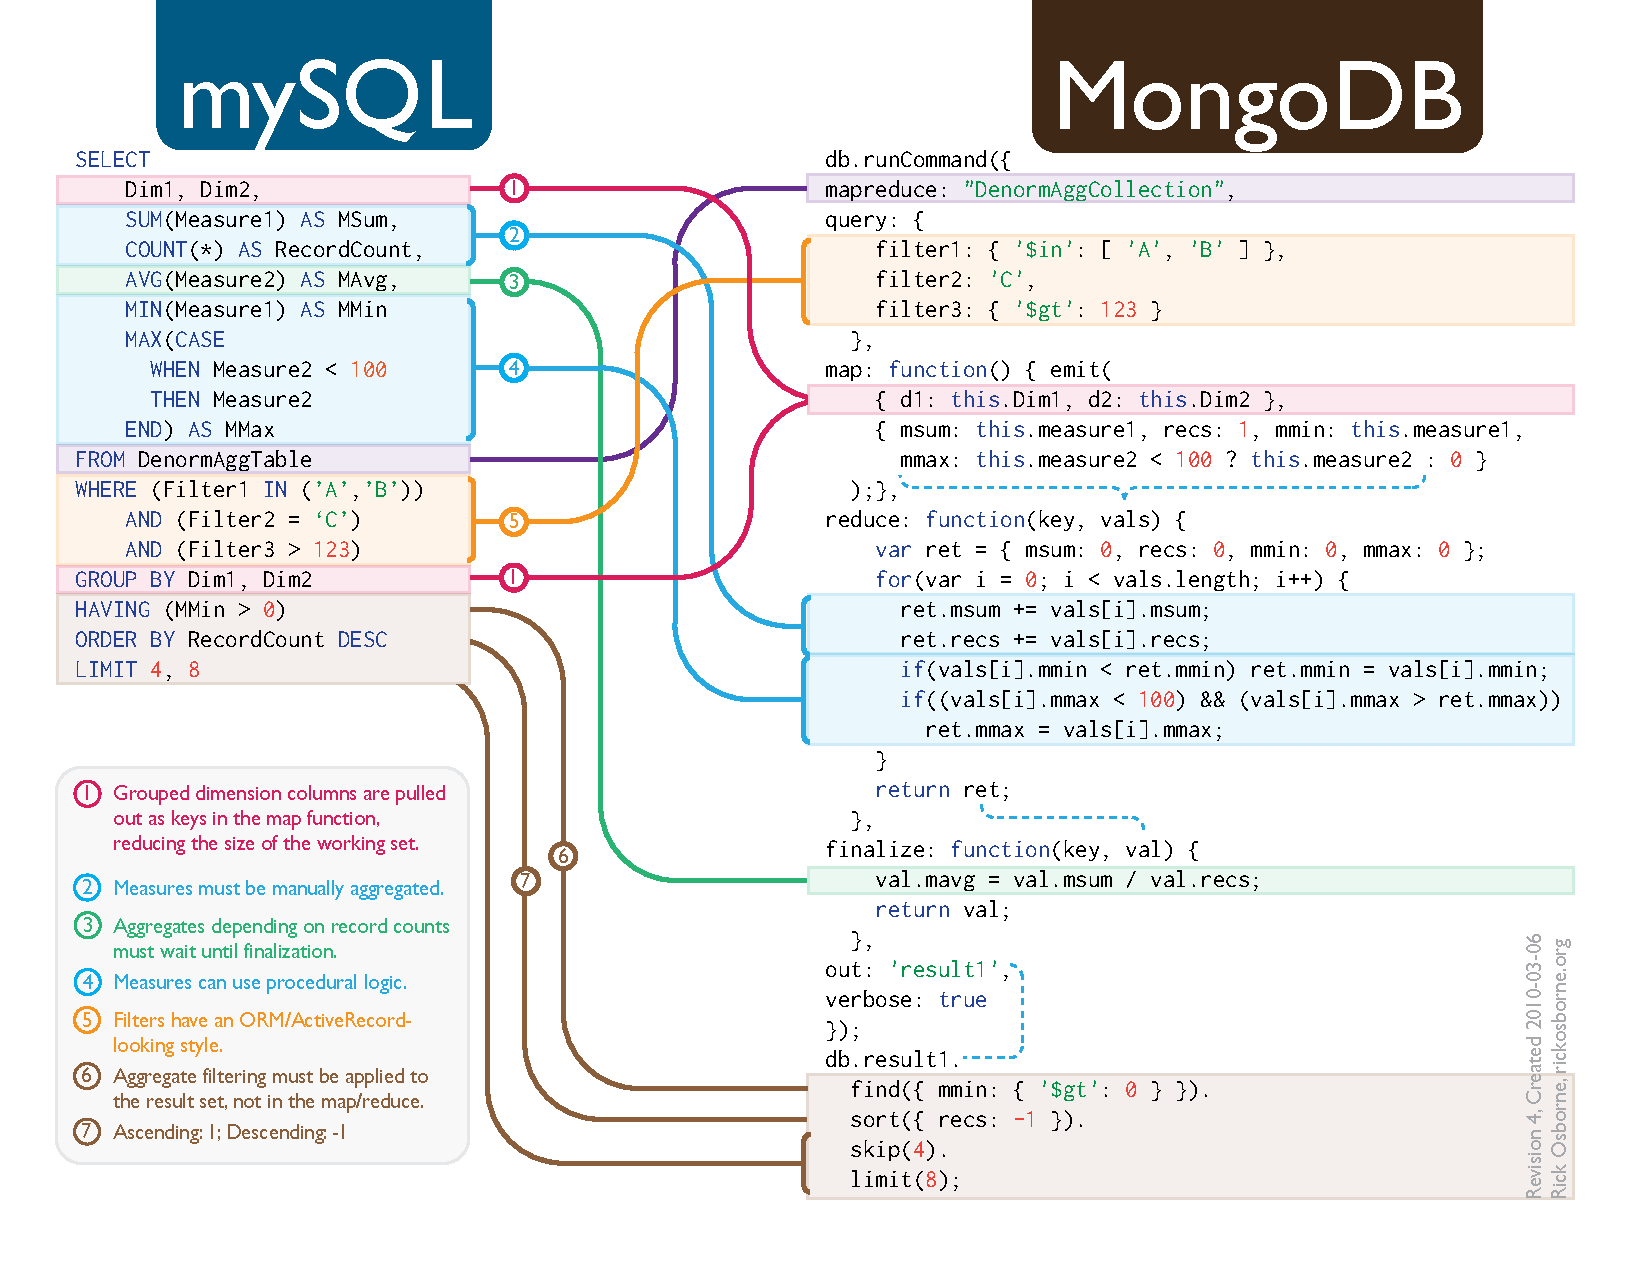
\includegraphics[width=0.7\textheight]{images/SQL-to-MongoDB.pdf}}{Sommige NoSQL systemen --- zoals MongoDB --- beschikken zoals te zien valt in deze afbeelding over dezelfde analytische kracht als een SQL database. De performantiekarakteristieken zijn echter verschillend. Afbeelding gebruikt met toestemming~\cite{sqlnosql}}{fig:sqlmongo}
\end{center}

%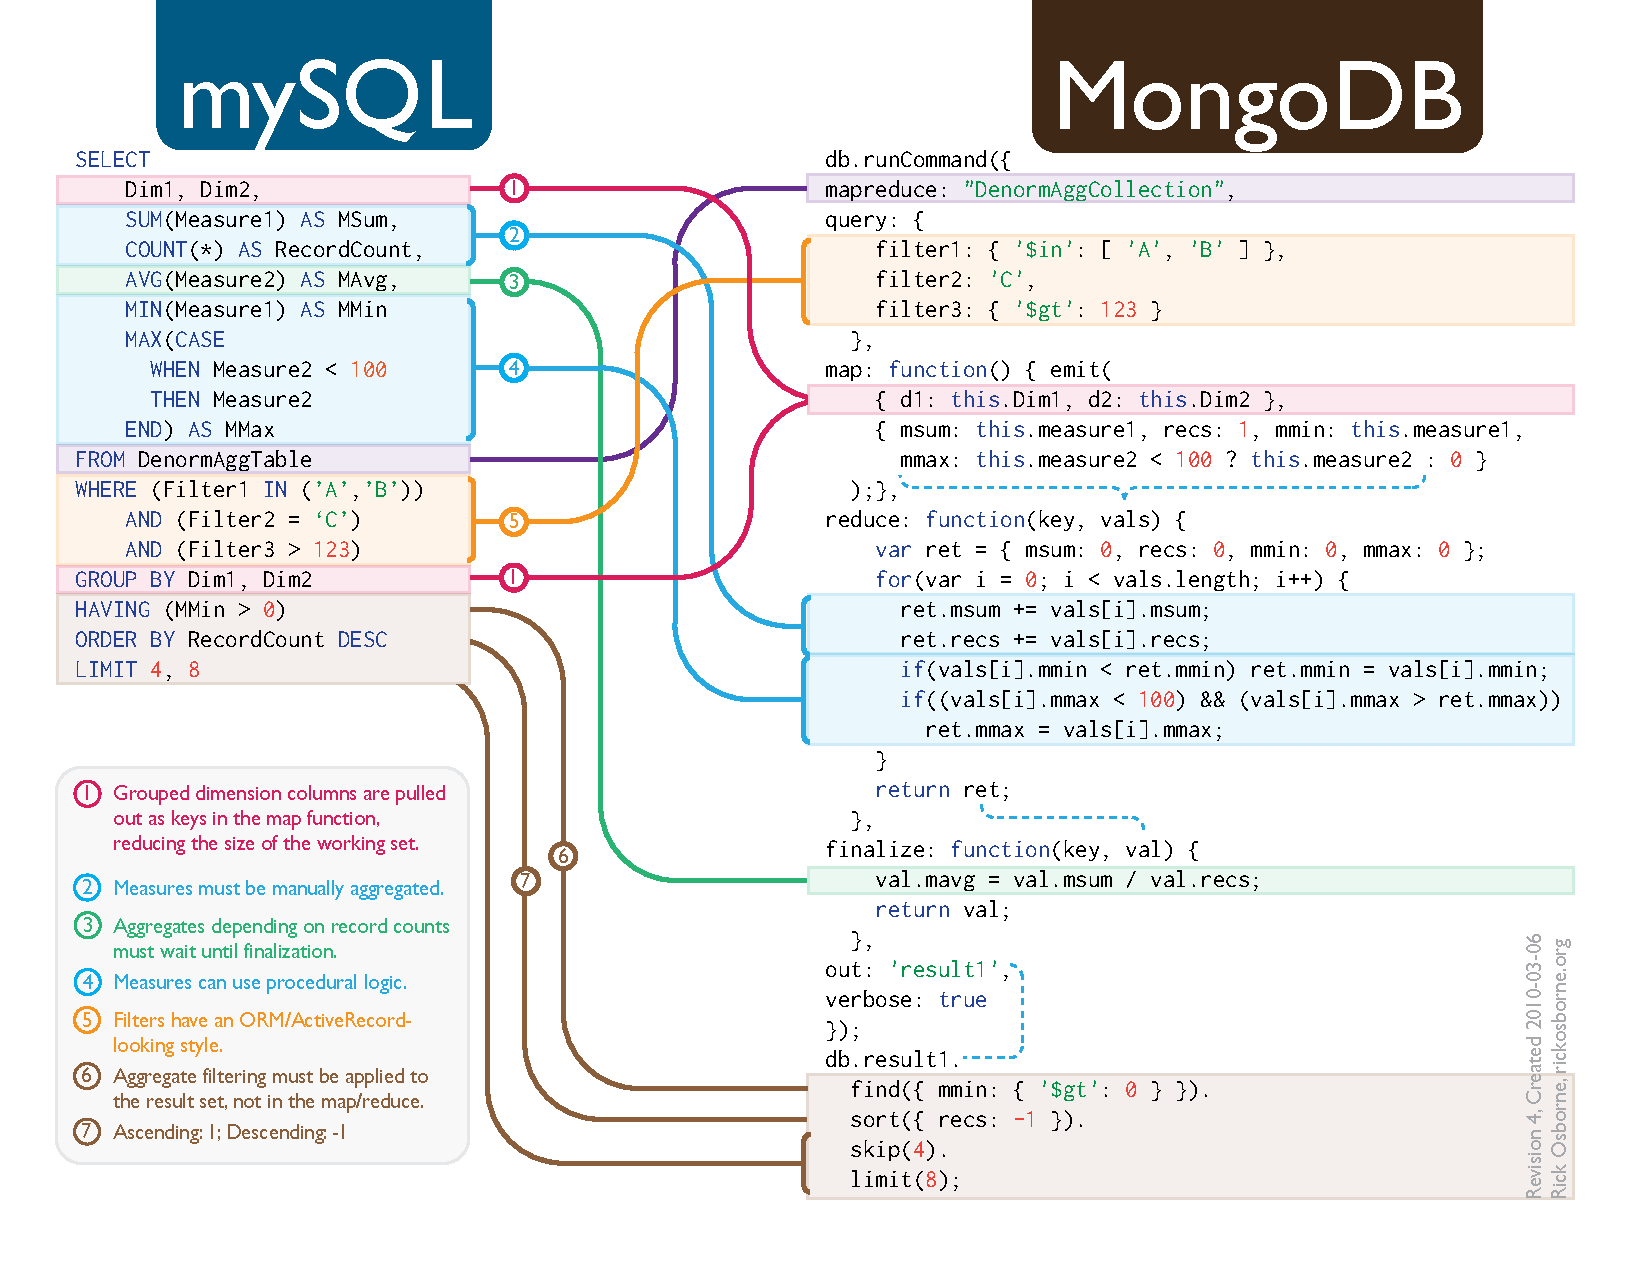
\includegraphics[width=0.8\textheight]{images/SQL-to-MongoDB.pdf}
%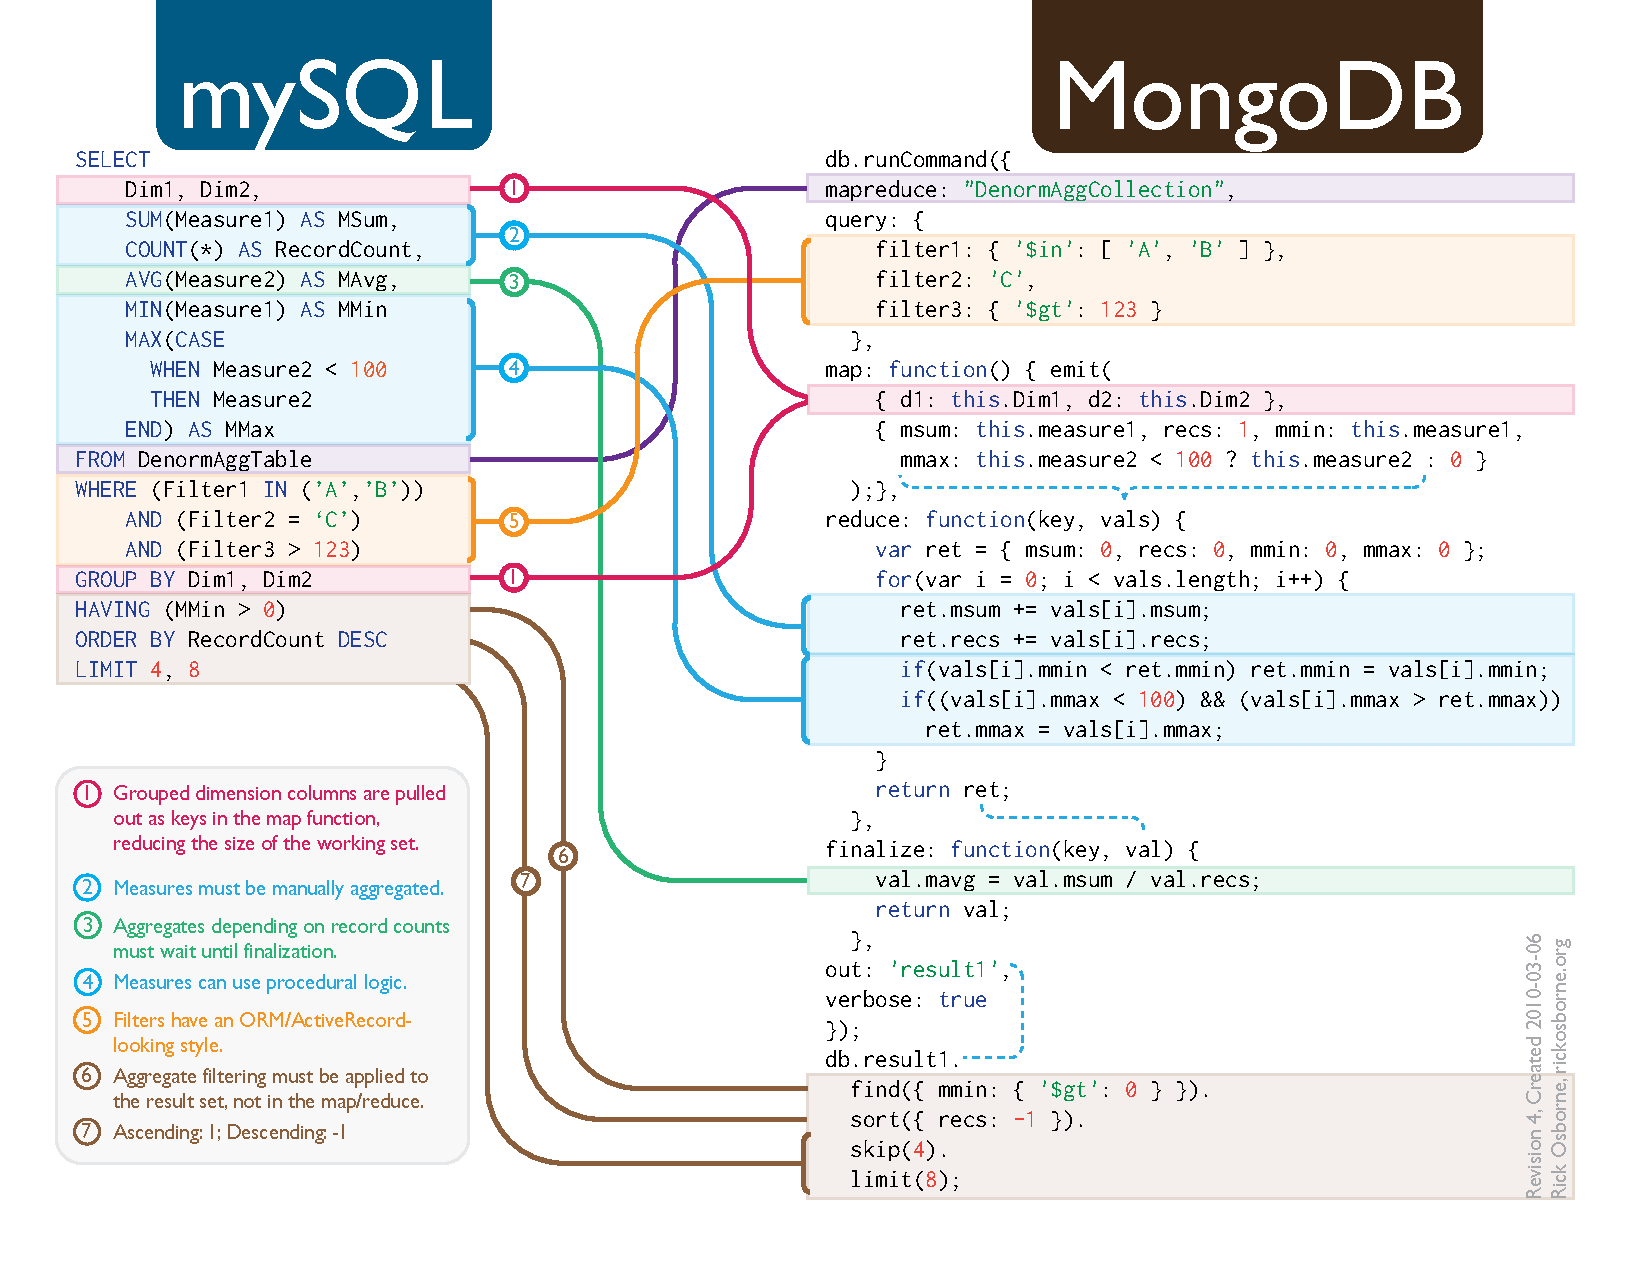
\includepdf{images/SQL-to-MongoDB.pdf}

\section{Componenten}
\hvFloat[
%floatPos=h,
nonFloat=true,
capWidth=1,%
capPos=b,%
rotAngle=90,%
objectPos=c%
]{figure}{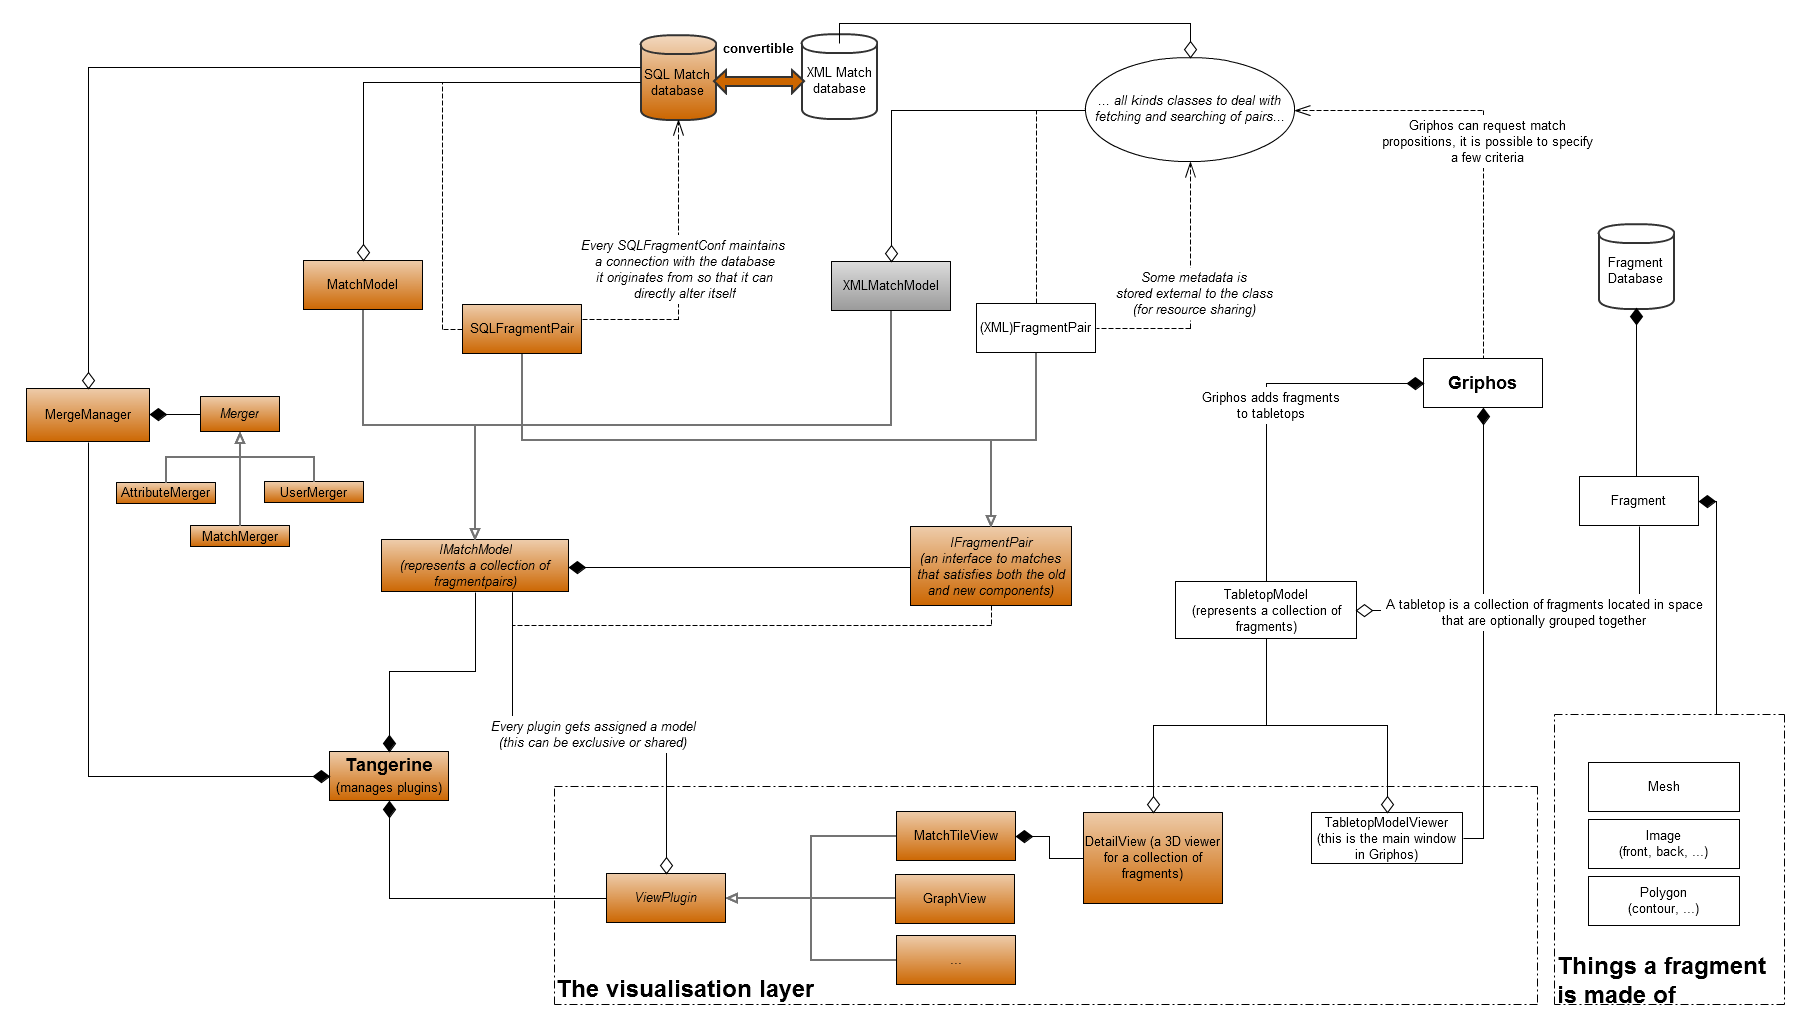
\includegraphics[width=0.95\textheight]{images/Bigtang.png}}{Een ruw overzicht van de componenten in het project en hoe het interageert met het reeds bestaande systeem.}{fig:tangbig}


\clearpage